\documentclass[10pt]{beamer}

\usetheme[progressbar=frametitle]{metropolis}
\usepackage{appendixnumberbeamer}
\usepackage{graphicx}
\usepackage{booktabs}
\usepackage{xspace}
\newcommand{\themename}{\textbf{\textsc{metropolis}}\xspace}


\title
{
Parallel CRC Algorithm and Implementation with CUDA
}
\date{\today}
\author{Mirco De Marchi - VR445319 \and Luigi Capogrosso - VR445456}
\institute{University of Verona -  Department of Computer Science}
\titlegraphic{\hfill
\includegraphics[height=1.5cm]{figures/UNIVR-logp.png}}


\begin{document}


\maketitle


\begin{frame}{Table of contents}
\setbeamertemplate{section in toc}[sections numbered]
\tableofcontents%[hideallsubsections]
\end{frame}


\section[Introduction]{Introduction}

\begin{frame}[fragile]{What is CRC}
\begin{figure}
\centering
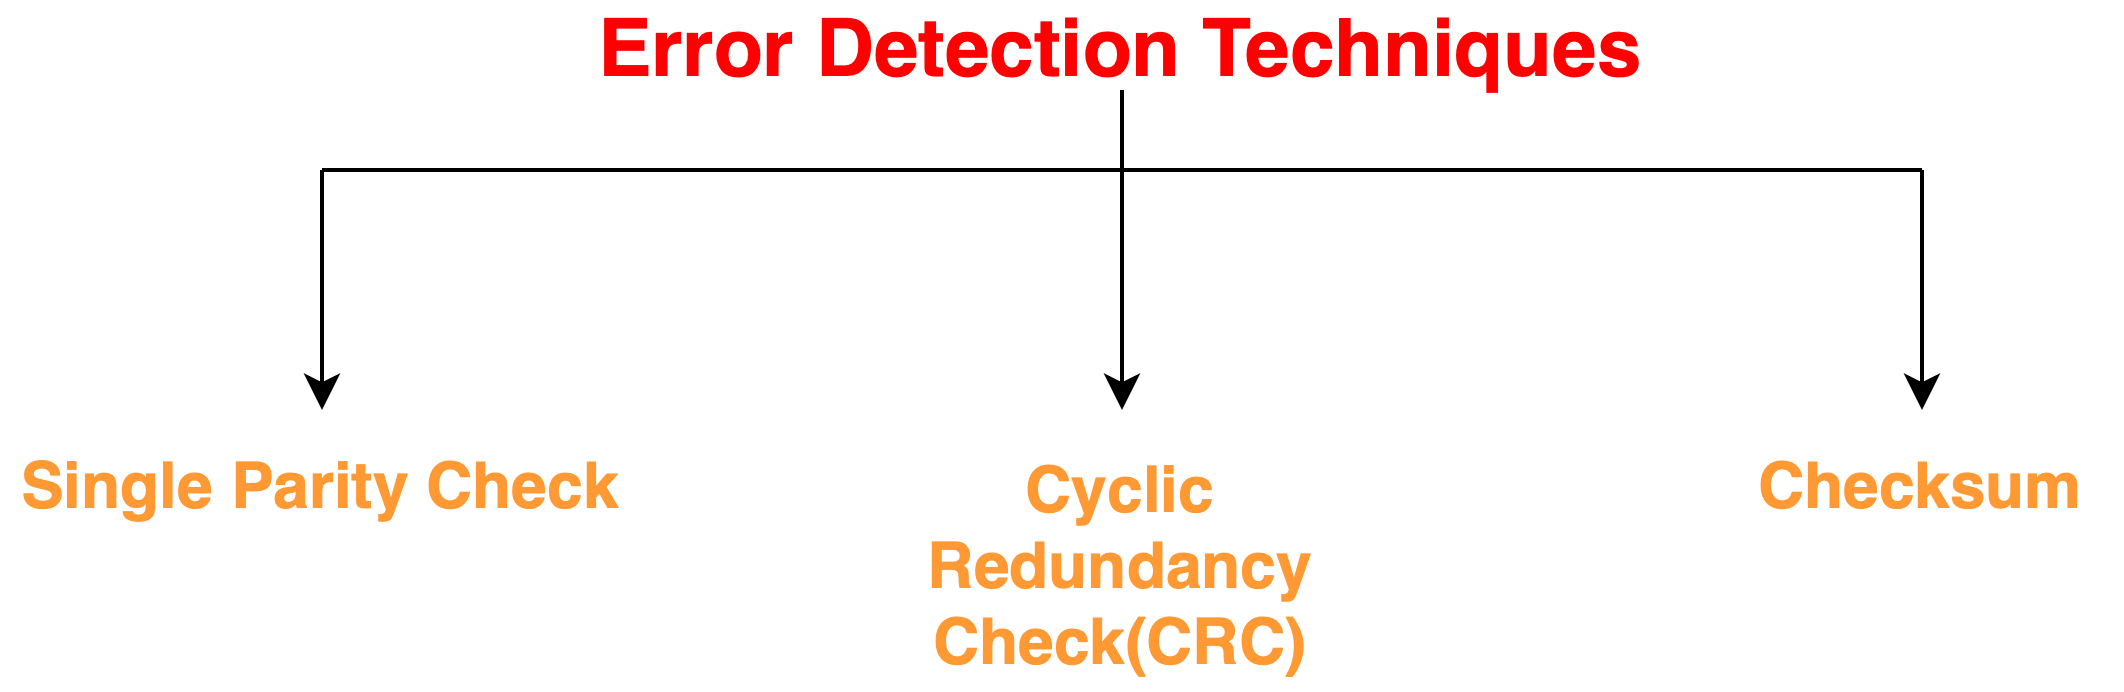
\includegraphics[width=\columnwidth]{figures/EDT.png}
\label{fig:EDT}
\end{figure}

Cyclic redundancy-check codes (\textbf{CRC codes}) are used for 
\textbf{detecting errors} that occur during trasmission \textbf{of digital 
(binary) information}.
\end{frame}


\begin{frame}[fragile]{Specification of a CRC code}
\begin{itemize}
\item CRCs are based on the theory of \textbf{systematic cyclic codes}, 
which encode messages by adding a fixed-length check value.

\item Specification of a CRC code requires definition so-called 
\textbf{generator polynomial}.

\item This polynomial becomes the \textbf{divisor} in a 
\textbf{polynomial long division}, which takes the message as the 
\textbf{divident} and in which the \textbf{quotient} is discarded and the 
\textbf{remainder} becomes the result.
\end{itemize}
\end{frame}


\begin{frame}[fragile]{Math Background}
\begin{itemize}
\item The CRC see the \textbf{message $A$} of \textbf{length $n$} as a 
\textbf{polynomial $A(x)$ of degree $n-1$} in which every bit of message 
is the coefficient of the respective monomial:
\[
   A=[a_{n-1},a_{n-2},\dots{},a_{2},a_{1},a_{0}]
\]
\[
   A(x)=a_{n-1}x^{n-1}+a_{n-2}x^{n-2}+\dots{}+a_{2}x^{2}+a_{1}x+a_{0}
\]

\item For example, the input data \verb|Ox25 = 0010 0101| is taken as:
\[
   A(x)=0x^{7}+0x^{6}+1x^{5}+0x^{4}+0x^{3}+1x^{2}+0x^{1}+1x^{0}
\]
\end{itemize}
\end{frame}


\begin{frame}[fragile]{Math Background cont.}
\begin{itemize}
\item Then for the CRC computation is used a 
\textbf{polynomial generator $G(x)$} that is 
\textbf{polynomial of degree $m$}. The major index coefficient is always 
1 $1$, in this way the polynomial generator guarantees to always be 
of $m$ degree.

\item In a reverse way the than the message $A$, \textbf{the polynomial 
generator can be represented as a sequence of bit $G$ of size $m+1$} 
with the most significant bit always to $1$.
\[
   G=[g_{m},g_{m-1},\dots{},g_{1},g_{0}] 
\]
\[
   G=g_{m}x^{m}+g_{m-1}x^{m-1}+\dots{}+g_{1}x+g_{0}
\]

\item For example, Ethernet uses the following 32-bit polynomial value:
\begin{gather*}
   G(x)=1+x+x^{2}+x^{4}+x^{5}+x^{7}+x^{8}+x^{10}+x^{11}+x^{12}+x^{16} \\
   +x^{22}+x^{23}+x^{26}+x^{32}
\end{gather*}
\end{itemize}
\end{frame}


\begin{frame}[fragile]{Math Background cont.}
\begin{itemize}
\item The \textbf{CRC} detection code \textbf{is the result of the reminder} 
after dividing the original message $A$ concatenated with $m$ zero bits 
by a polynomial generator in \textbf{binary modulo 2 arithmetic}.

\item In the polynomial version this definition of CRC is equivalent to:
\[
   CRC[A(x)]=A(x)x^{m}mod2(G(x))
\]
\end{itemize}
\end{frame}


\section[CRC algorithms]{CRC algorithms}

\begin{frame}[fragile]{Bitwise CRC algorithm}
\begin{verbatim}
// Result size: N + M.
append(message, M)

// Usually 0.
message[M-1 : 0] = crc_initial_value

// Check each bit of the message.
for i in range(0 : N) 
{
   LSB = (N + M - 1) - i
   if (message[LSB] == 1)
   {
      message[LSB : LSB-(M-1)] ^= 
      polynomial_generator;
   }
}

return message[M-1 : 0];
\end{verbatim}
\end{frame}


\begin{frame}[fragile]{The CRC lookup table optimization}
\begin{scriptsize}
\begin{verbatim}
const uint32_t crc32_tab[] = {
   0x00000000, 0x77073096, 0xee0e612c, 0x990951ba, 0x076dc419, 0x706af48f,
   0xe963a535, 0x9e6495a3, 0x0edb8832, 0x79dcb8a4, 0xe0d5e91e, 0x97d2d988,
   0x09b64c2b, 0x7eb17cbd, 0xe7b82d07, 0x90bf1d91, 0x1db71064, 0x6ab020f2,
   0xf3b97148, 0x84be41de, 0x1adad47d, 0x6ddde4eb, 0xf4d4b551, 0x83d385c7,
   0x136c9856, 0x646ba8c0, 0xfd62f97a, 0x8a65c9ec, 0x14015c4f, 0x63066cd9,
   0xfa0f3d63, 0x8d080df5, 0x3b6e20c8, 0x4c69105e, 0xd56041e4, 0xa2677172,
   0x3c03e4d1, 0x4b04d447, 0xd20d85fd, 0xa50ab56b, 0x35b5a8fa, 0x42b2986c,
   0xdbbbc9d6, 0xacbcf940, 0x32d86ce3, 0x45df5c75, 0xdcd60dcf, 0xabd13d59,
   0x26d930ac, 0x51de003a, 0xc8d75180, 0xbfd06116, 0x21b4f4b5, 0x56b3c423,
   0xcfba9599, 0xb8bda50f, 0x2802b89e, 0x5f058808, 0xc60cd9b2, 0xb10be924,
   0x2f6f7c87, 0x58684c11, 0xc1611dab, 0xb6662d3d, 0x76dc4190, 0x01db7106,
   0x98d220bc, 0xefd5102a, 0x71b18589, 0x06b6b51f, 0x9fbfe4a5, 0xe8b8d433,
   0x7807c9a2, 0x0f00f934, 0x9609a88e, 0xe10e9818, 0x7f6a0dbb, 0x086d3d2d,
   0x91646c97, 0xe6635c01, 0x6b6b51f4, 0x1c6c6162, 0x856530d8, 0xf262004e,
   0x6c0695ed, 0x1b01a57b, 0x8208f4c1, 0xf50fc457, 0x65b0d9c6, 0x12b7e950,
   0x8bbeb8ea, 0xfcb9887c, 0x62dd1ddf, 0x15da2d49, 0x8cd37cf3, 0xfbd44c65,
   0x4db26158, 0x3ab551ce, 0xa3bc0074, 0xd4bb30e2, 0x4adfa541, 0x3dd895d7,
   0xa4d1c46d, 0xd3d6f4fb, 0x4369e96a, 0x346ed9fc, 0xad678846, 0xda60b8d0,
   0x44042d73, 0x33031de5, 0xaa0a4c5f, 0xdd0d7cc9, 0x5005713c, 0x270241aa,
   0xbe0b1010, 0xc90c2086, 0x5768b525, 0x206f85b3, 0xb966d409, 0xce61e49f,
   0x5edef90e, 0x29d9c998, 0xb0d09822, 0xc7d7a8b4, 0x59b33d17, 0x2eb40d81,
   0xb7bd5c3b, 0xc0ba6cad, 0xedb88320, 0x9abfb3b6, 0x03b6e20c, 0x74b1d29a,
\end{verbatim}
\end{scriptsize}
\end{frame}


\begin{frame}[fragile]{The CRC lookup table optimization}   
\begin{scriptsize}
\begin{verbatim}
   0xead54739, 0x9dd277af, 0x04db2615, 0x73dc1683, 0xe3630b12, 0x94643b84,
   0x0d6d6a3e, 0x7a6a5aa8, 0xe40ecf0b, 0x9309ff9d, 0x0a00ae27, 0x7d079eb1,
   0xf00f9344, 0x8708a3d2, 0x1e01f268, 0x6906c2fe, 0xf762575d, 0x806567cb,
   0x196c3671, 0x6e6b06e7, 0xfed41b76, 0x89d32be0, 0x10da7a5a, 0x67dd4acc,
   0xf9b9df6f, 0x8ebeeff9, 0x17b7be43, 0x60b08ed5, 0xd6d6a3e8, 0xa1d1937e,
   0x38d8c2c4, 0x4fdff252, 0xd1bb67f1, 0xa6bc5767, 0x3fb506dd, 0x48b2364b,
   0xd80d2bda, 0xaf0a1b4c, 0x36034af6, 0x41047a60, 0xdf60efc3, 0xa867df55,
   0x316e8eef, 0x4669be79, 0xcb61b38c, 0xbc66831a, 0x256fd2a0, 0x5268e236,
   0xcc0c7795, 0xbb0b4703, 0x220216b9, 0x5505262f, 0xc5ba3bbe, 0xb2bd0b28,
   0x2bb45a92, 0x5cb36a04, 0xc2d7ffa7, 0xb5d0cf31, 0x2cd99e8b, 0x5bdeae1d,
   0x9b64c2b0, 0xec63f226, 0x756aa39c, 0x026d930a, 0x9c0906a9, 0xeb0e363f,
   0x72076785, 0x05005713, 0x95bf4a82, 0xe2b87a14, 0x7bb12bae, 0x0cb61b38,
   0x92d28e9b, 0xe5d5be0d, 0x7cdcefb7, 0x0bdbdf21, 0x86d3d2d4, 0xf1d4e242,
   0x68ddb3f8, 0x1fda836e, 0x81be16cd, 0xf6b9265b, 0x6fb077e1, 0x18b74777,
   0x88085ae6, 0xff0f6a70, 0x66063bca, 0x11010b5c, 0x8f659eff, 0xf862ae69,
   0x616bffd3, 0x166ccf45, 0xa00ae278, 0xd70dd2ee, 0x4e048354, 0x3903b3c2,
   0xa7672661, 0xd06016f7, 0x4969474d, 0x3e6e77db, 0xaed16a4a, 0xd9d65adc,
   0x40df0b66, 0x37d83bf0, 0xa9bcae53, 0xdebb9ec5, 0x47b2cf7f, 0x30b5ffe9,
   0xbdbdf21c, 0xcabac28a, 0x53b39330, 0x24b4a3a6, 0xbad03605, 0xcdd70693,
   0x54de5729, 0x23d967bf, 0xb3667a2e, 0xc4614ab8, 0x5d681b02, 0x2a6f2b94,
   0xb40bbe37, 0xc30c8ea1, 0x5a05df1b, 0x2d02ef8d
};
\end{verbatim}
\end{scriptsize}
\end{frame}


\begin{frame}[fragile]{Bytewise CRC algorithm}
\begin{verbatim}
// Result size: N + M.
append(message, M)

// Usually 0
message[M-1 : 0] = crc_initial_value

// Check each byte of the message.
for i in range(0:N / 8-1) 
{
   LSB = (N + M - 1) - (i * 8);
   message[LSB-8 : LSB-8-(M-1)] ^= 
   lookup_table[message[LSB : LSB-7]];
}

return message[M-1 : 0];
\end{verbatim}
\end{frame}


\section[Implementation]{Implementation}

\begin{frame}[fragile]{Parallel CRC algorithm}
\begin{itemize}
\item For a given message with any length, we \textbf{first chunk the 
message into blocks}, each of which has a fixed size equal to the degree of 
the generator polynomial. 

\item The message is seen as divided in M bit size chunk and the following 
is its polynomial representation:
\[
   A(x)=W_{n-1}(x)x^{(n-1)M}+\dots{}+W_{1}(x)x^{M}+W_{0}(x)
\]

\item Where each $W_{i}(x)$ polynomial is a chunk of the message. 
From this equation and the CRC definition, we can compute the CRC for the 
chunked message by:
\[
   CRC[A(x)]=W_{n-1}x^{nM}modG(x)+\dots{}+W_{0}x^{M}modG(x)
\]
\end{itemize}
\end{frame}

\begin{frame}[fragile]{Parallel CRC algorithm cont.}
\begin{itemize}
\item Furthermore, from the Galois Field operations lemma, we obtain that:
\[
\begin{split}
W_{i}(x)x^{(i+1)M}modG(x) = & (W_{i}(x)modG(x) \\& x^{(i+1)M}modG(x))modG(x)
\end{split}
\]

\item The degree of the polynomial $W_{i}(x)$ for each chunk is $M-1$, 
therefore it is less than $M$, it means that $W_{i}(x)modG(x)=W_{i}(x)$. 
On the other hand the beta coefficients are defined 
as $\beta{}_{i}=x^{(i+1)*M}modG(x)$ for $i=0,1,\dots{},n-1$. 
Therefore we have:
\[
   CRC[A(x)]=W_{n-1}\otimes{}\beta{}_{n-1}\oplus{}\dots{}
   \oplus{}W_{0}\otimes{}\beta{}_{0}
\]
\end{itemize}

Note that the operations $\otimes{}$, $\oplus{}$ in the above equation is 
Galois Field multiplication, addition over $GF(2^{M})$, respectively.
\end{frame}

\begin{frame}[fragile]{Parallel CRC algorithm cont.}
\begin{figure}[bt]
\centering
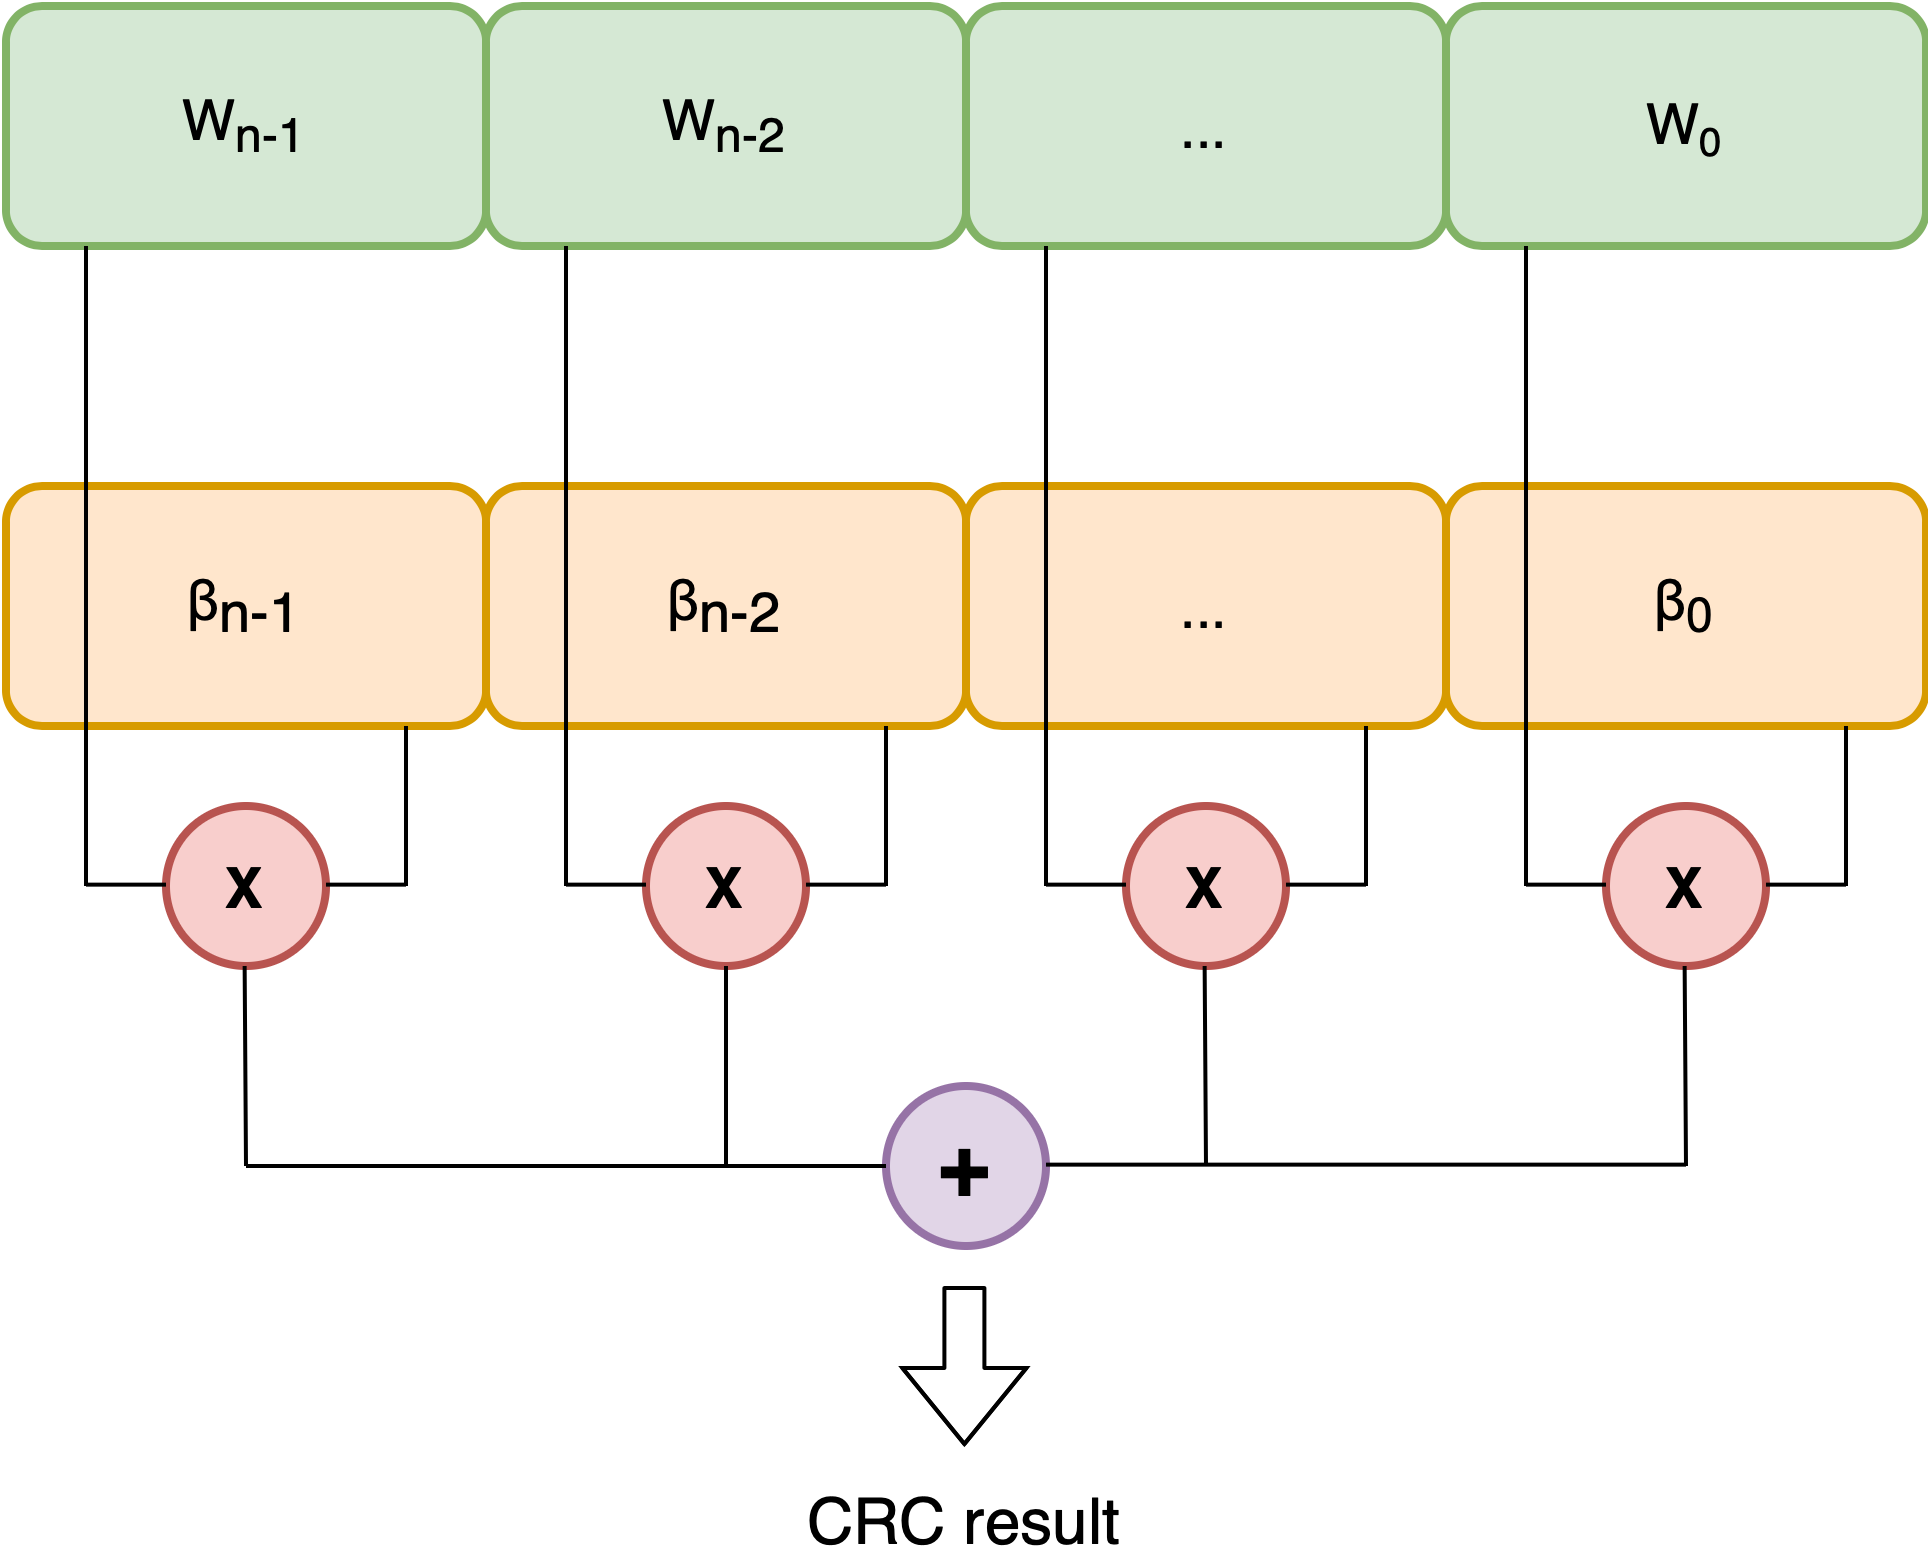
\includegraphics[width=7cm]{figures/PCRC.png}
\caption{ILLUSTRATION OF  PARALLEL CRC ALGORITHM OVER CHUNK OF M BITS}
\label{fig:PCRC}
\end{figure}
\end{frame}

\begin{frame}[fragile]{Threads execution}
\begin{verbatim}
// Get the data of this thread.
W_i = orginal_message[global_index];
beta_i = beta[global_index];

// Perform binary modulo 2 multiplication.
mul = mod2_mul(W_i, beta_i);

// Perform binary modulo 2 reminder.
mod = mod2_mod(mul, generator_poly);

// Copy in shared memory.
shared_memory[threadX] = mod;
sync();

// XOR all data in shared memory.
return xored(shared_memory);
\end{verbatim}
\end{frame}

\begin{frame}[fragile]{Threads execution cont.}
\begin{figure}[bt]
\centering
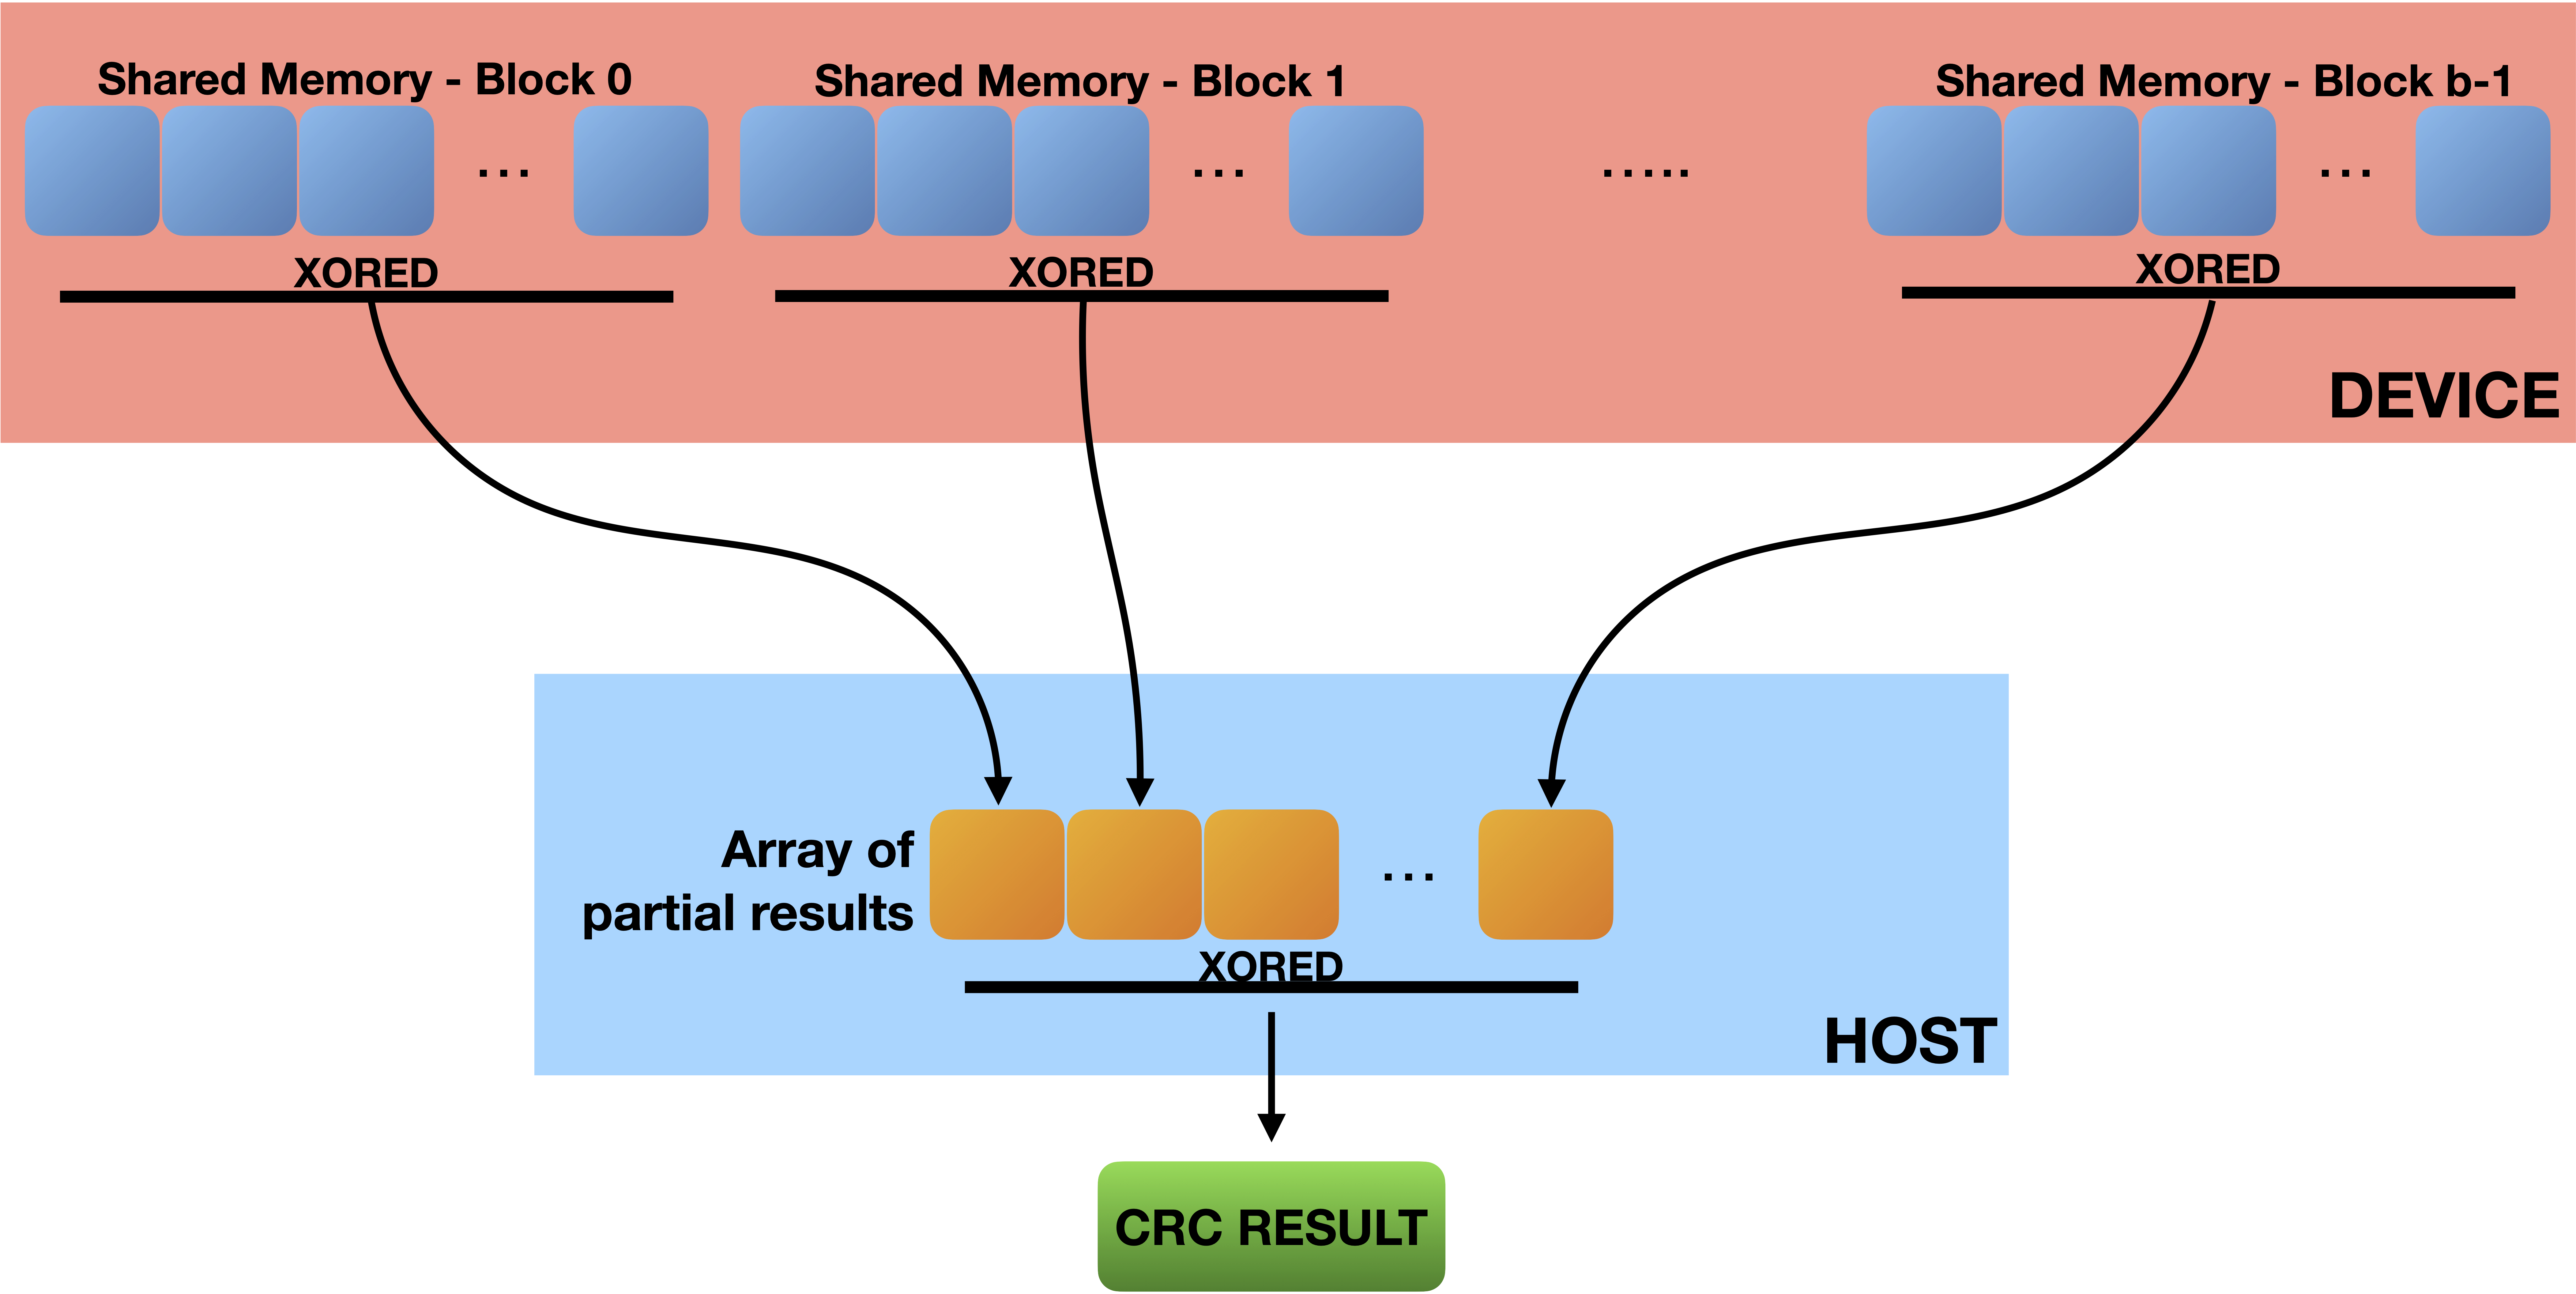
\includegraphics[width=7cm]{figures/PCRC-reduction.png}
\caption{XOR OPERATIONS PERFORM BY DEVICE IN RELATION WITH THE ONE PERFORM BY HOST}
\label{fig:PCRC-reduction}
\end{figure}
\end{frame}

\section[Performance analysis]{Performance analysis}


\begin{frame}[fragile]{Test PCRC 64 blocksize}
$N=2^{16}$. $BlockSize=64$. $StreamDim=4$. $SegSize=N/StreamDim$
\begin{footnotesize}
\begin{tabular}{l|l|l|l|l|r|r|r|r|r|r||c|c|}
\toprule
\textbf{Test PCRC 64 blocksize} & \textbf{Speedup} \\
\midrule
PCRC8                                           &	34.71340 \\
PCRC8 with reduction                            &	37.40804 \\
PCRC8 with task parallelism                     &	27.86828 \\
PCRC8 bytewise comparison                       &	2.58712  \\
PCRC8 bytewise comparison with reduction:       &	2.61057  \\
PCRC8 bytewise comparison with task parallelism &	1.93434  \\
PCRC16                                           &	34.98040 \\
PCRC16 with reduction                            &	40.59672 \\
PCRC16 with task parallelism                     &	26.11727 \\
PCRC16 bytewise comparison                       &	3.44060  \\
PCRC16 bytewise comparison with reduction:       &	3.85280  \\
PCRC16 bytewise comparison with task parallelism &	1.51222  \\
PCRC32                                           &	20.23205 \\
PCRC32 with reduction                            &	20.01593 \\
PCRC32 with task parallelism                     &	8.46386  \\
PCRC32 bytewise comparison                       &	1.78715  \\
PCRC32 bytewise comparison with reduction:       &	1.86166  \\
PCRC32 bytewise comparison with task parallelism &	0.71914  \\
\bottomrule
\end{tabular}
\end{footnotesize}
\end{frame}

\begin{frame}[fragile]{Test PCRC 128 blocksize}
$N=2^{16}$. $BlockSize=128$. $StreamDim=4$. $SegSize=N/StreamDim$
\begin{footnotesize}
\begin{tabular}{l|l|l|l|l|r|r|r|r|r|r||c|c|}
\toprule
\textbf{Test PCRC 128 blocksize} & \textbf{Speedup} \\
\midrule
PCRC8                                           &	34.63720 \\
PCRC8 with reduction                            &	37.41059 \\
PCRC8 with task parallelism                     &	28.19650 \\
PCRC8 bytewise comparison                       &	2.24552  \\
PCRC8 bytewise comparison with reduction:       &	2.70207  \\
PCRC8 bytewise comparison with task parallelism &	2.02773  \\
PCRC16                                           &	34.14637 \\
PCRC16 with reduction                            &	40.48397 \\
PCRC16 with task parallelism                     &	25.37525 \\
PCRC16 bytewise comparison                       &	3.57066  \\
PCRC16 bytewise comparison with reduction:       &	3.60613  \\
PCRC16 bytewise comparison with task parallelism &	1.49754  \\
PCRC32                                           &	20.41607 \\
PCRC32 with reduction                            &	21.54121 \\
PCRC32 with task parallelism                     &	8.51250  \\
PCRC32 bytewise comparison                       &	1.89645  \\
PCRC32 bytewise comparison with reduction:       &	1.85455  \\
PCRC32 bytewise comparison with task parallelism &	0.79350  \\
\bottomrule
\end{tabular}
\end{footnotesize}
\end{frame}

\begin{frame}[fragile]{Test PCRC 256 blocksize}
$N=2^{16}$. $BlockSize=256$. $StreamDim=4$. $SegSize=N/StreamDim$
\begin{footnotesize}
\begin{tabular}{l|l|l|l|l|r|r|r|r|r|r||c|c|}
\toprule
\textbf{Test PCRC 256 blocksize} & \textbf{Speedup} \\
\midrule
PCRC8                                           &	35.11670 \\
PCRC8 with reduction                            &	37.36065 \\
PCRC8 with task parallelism                     &	29.85230 \\
PCRC8 bytewise comparison                       &	2.66612  \\
PCRC8 bytewise comparison with reduction:       &	2.71714  \\
PCRC8 bytewise comparison with task parallelism &	2.00425  \\
PCRC16                                           &	33.09628 \\
PCRC16 with reduction                            &	39.25975 \\
PCRC16 with task parallelism                     &	27.58368 \\
PCRC16 bytewise comparison                       &	3.53824  \\
PCRC16 bytewise comparison with reduction:       &	3.66416  \\
PCRC16 bytewise comparison with task parallelism &	1.54122  \\
PCRC32                                           &	20.29566 \\
PCRC32 with reduction                            &	21.39834 \\
PCRC32 with task parallelism                     &	7.98474  \\
PCRC32 bytewise comparison                       &	1.75776  \\
PCRC32 bytewise comparison with reduction:       &	1.80291  \\
PCRC32 bytewise comparison with task parallelism &	0.68456  \\
\bottomrule
\end{tabular}
\end{footnotesize}
\end{frame}

\begin{frame}[fragile]{Test PCRC 128 blocksize}
$N=2^{16}$. $BlockSize=128$. $StreamDim=2$. $SegSize=N/StreamDim$
\begin{footnotesize}
\begin{tabular}{l|l|l|l|l|r|r|r|r|r|r||c|c|}
\toprule
\textbf{Test PCRC 128 blocksize} & \textbf{Speedup} \\
\midrule
PCRC8                                           &	21.32339 \\
PCRC8 with reduction                            &	39.41265 \\
PCRC8 with task parallelism                     &	32.97171 \\
PCRC8 bytewise comparison                       &	2.70535  \\
PCRC8 bytewise comparison with reduction:       &	2.64768  \\
PCRC8 bytewise comparison with task parallelism &	2.48787  \\
PCRC16                                           &	33.66302 \\
PCRC16 with reduction                            &	38.77745 \\
PCRC16 with task parallelism                     &	30.44083 \\
PCRC16 bytewise comparison                       &	3.46636  \\
PCRC16 bytewise comparison with reduction:       &	3.59283  \\
PCRC16 bytewise comparison with task parallelism &	2.80089  \\
PCRC32                                           &	20.42403 \\
PCRC32 with reduction                            &	21.38471 \\
PCRC32 with task parallelism                     &	7.35099  \\
PCRC32 bytewise comparison                       &	1.87434  \\
PCRC32 bytewise comparison with reduction:       &	1.86528  \\
PCRC32 bytewise comparison with task parallelism &	0.72902  \\
\bottomrule
\end{tabular}
\end{footnotesize}
\end{frame}

\begin{frame}[fragile]{Test PCRC 128 blocksize}
$N=2^{16}$. $BlockSize=128$. $StreamDim=8$. $SegSize=N/StreamDim$
\begin{footnotesize}
\begin{tabular}{l|l|l|l|l|r|r|r|r|r|r||c|c|}
\toprule
\textbf{Test PCRC 128 blocksize} & \textbf{Speedup} \\
\midrule
PCRC8                                           &	35.05756 \\
PCRC8 with reduction                            &	38.59024 \\
PCRC8 with task parallelism                     &	11.97966 \\
PCRC8 bytewise comparison                       &	2.65855  \\
PCRC8 bytewise comparison with reduction:       &	2.73349  \\
PCRC8 bytewise comparison with task parallelism &	1.20074  \\
PCRC16                                           &	34.06469 \\
PCRC16 with reduction                            &	38.96202 \\
PCRC16 with task parallelism                     &	11.68695 \\
PCRC16 bytewise comparison                       &	3.87572  \\
PCRC16 bytewise comparison with reduction:       &	3.22093  \\
PCRC16 bytewise comparison with task parallelism &	1.58960  \\
PCRC32                                           &	20.83102 \\
PCRC32 with reduction                            &	22.14467 \\
PCRC32 with task parallelism                     &	6.38649  \\
PCRC32 bytewise comparison                       &	1.94807  \\
PCRC32 bytewise comparison with reduction:       &	1.91344  \\
PCRC32 bytewise comparison with task parallelism &	0.65893  \\
\bottomrule
\end{tabular}
\end{footnotesize}
\end{frame}

\begin{frame}[fragile]{Test PCRC 128 blocksize}
$N=2^{16}$. $BlockSize=128$. $StreamDim=4$. $SegSize=N/8$
\begin{footnotesize}
\begin{tabular}{l|l|l|l|l|r|r|r|r|r|r||c|c|}
\toprule
\textbf{Test PCRC 128 blocksize} & \textbf{Speedup} \\
\midrule
PCRC8                                           &	35.41841 \\
PCRC8 with reduction                            &	40.88182 \\
PCRC8 with task parallelism                     &	17.13281 \\
PCRC8 bytewise comparison                       &	2.40438  \\
PCRC8 bytewise comparison with reduction:       &	2.97784  \\
PCRC8 bytewise comparison with task parallelism &	0.47928  \\
PCRC16                                           &	34.66451 \\
PCRC16 with reduction                            &	42.29803 \\
PCRC16 with task parallelism                     &	16.70620 \\
PCRC16 bytewise comparison                       &	4.04358  \\
PCRC16 bytewise comparison with reduction:       &	3.76574  \\
PCRC16 bytewise comparison with task parallelism &	1.51226  \\
PCRC32                                           &	21.27053 \\
PCRC32 with reduction                            &	21.97304 \\
PCRC32 with task parallelism                     &	7.47568  \\
PCRC32 bytewise comparison                       &	1.92987  \\
PCRC32 bytewise comparison with reduction:       &	1.90569  \\
PCRC32 bytewise comparison with task parallelism &	0.52763  \\
\bottomrule
\end{tabular}
\end{footnotesize}
\end{frame}

\begin{frame}[fragile]{Conclusion}
The implementation with tasks parallelism does not give better performance 
because the overhead of the technique is not positively compensated on the 
improvement that leads to performance. So the best result with parallelism 
tasks is obtained for $StreamDim=4$ and $SegSize=N/StreamDim$. 

In general the best performances are with $BlockSize=128$, while in the case of 
parallelism tasks the best performances are with $StreamDim=2$ and 
$SegSize=N/StreamDim$ using the reduction algorithm that reduces the divergence 
of the threads, which on average increases the performance compared to the 
standard solution of some speedup units.
\end{frame}


\end{document}